
In this thesis the single shot detector \ac{YOLO} \cite{yolov1} is used.
Single shot means that \ac{YOLO} produces class predictions as well as bounding box predictions in a single network pass.
In contrast to the other methods mentioned in \ref{sec:hostory_obj_detection}, this yields a huge improvement in performance and resource efficiency.
The \ac{YOLO} network, more precisely \ac{YOLOv4} \cite{yolov4} was selected, because it is currently the state-of-the-art in the commonly known object detection benchmarks.
Furthermore, there exists a version of \ac{YOLOv4} (YOLOv4-tiny \cite{yolov4_tiny}), which can be used in resource constrained environments such as mobile devices.

\subsubsection{General}

\ac{YOLOv4} unifies class prediction and bounding box regression in a single neural network.
It is an anchor based detection network and hence outputs regression offsets based on a predefined anchor box.
The architecture can be structured into three main parts: a backbone, a neck and a head.
The backbone receives as input an image and is responsible to extract features out of it.
Further, the neck receives the output of the backbone and produces output feature maps, which are further processed by the head to produce the final prediction.
The final prediction is then a vector with bounding box regression offsets for the anchors, an objectness score, which class agnostically indicates whether an object is present, as well as a vector of independent class probabilities.

\subsubsection{Backbone}

- TODO backbone is a smaller scale of the original Darknet53

The backbone of the \ac{YOLOv4} network is mostly formed out of YOLOConv layers (tab. \ref{tab:yoloconv}), which is sequentially build out of a convolutional layer, a batch normalization layer and a leaky \ac{ReLU} activation function, following the principles of \cite{batchnorm}.


The initial two layers (c0, c1) use an increased stride and a valid padding to first reduce the input size of the image.
The following layers always use three $3x3$ convolutions, followed by one $1x1$ convolution and a max pooling layer to half the feature map size.
The number of filters for the four convolutions is always $N * (K, K/2, K/2, K)$, where $N$ denotes the layer number and $K$ the number of filters beginning with $64$.
So as can be seen in \ref{tab:darknet_tiny_arch}, where the whole architecture of the backbone is presented, in the first layer the kernel sizes are set to $(64, 32, 32, 64)$.
Further, the backbone has three outputs, seen on the right of the table ($Skip_S$, $Skip_M$, $Skip_L$), which are used as skip connections to the following neck network.
$S$, $M$, $L$ indicates here the size of the detected object (small, medium, large).



\begin{table} %[H]
\begin{center}

\begin{tabular}{l|c|c|c|c|c|c|c}
    \textbf{Layer} & \textbf{Input} & \textbf{Type} & \textbf{Filters} & \textbf{Size} & \textbf{Stride} & \textbf{Padding} & \textbf{Output} \\
    \hline
    \textbf{Reduction Layer} & & & & & &\\
    c0 & img & YOLOConv & 32 & 3x3 & 2 & valid\\
    c1 & c0 & YOLOConv & 64 & 3x3 & 2 & valid\\
    \textbf{Layer 1} & & & & & &\\
    c2 & c1 & YOLOConv & 64 & 3x3 & 1 & same\\
    c3 & c2 & YOLOConv & 32 & 3x3 & 1 & same\\
    c4 & c3 & YOLOConv & 32 & 3x3 & 1 & same\\
    c5 & c3 \& c4 & YOLOConv & 64 & 1x1 & 1 & same\\
    m0 & c2 \& c5 & MaxPool &  & 2x2 & 2 & same\\
    \textbf{Layer 2} & & & & & &\\
    c6 & m0 & YOLOConv & 128 & 3x3 & 1 & same\\
    c7 & c6 & YOLOConv & 64 & 3x3 & 1 & same\\
    c8 & c7 & YOLOConv & 64 & 3x3 & 1 & same\\
    c9 & c7 \& c8 & YOLOConv & 128 & 1x1 & 1 & same & $Skip_S$\\
    m1 & c6 \& c9 & MaxPool & & 2x2  & 2 & same\\
    \textbf{Layer 3} & & & & & &\\
    c10 & m1 & YOLOConv & 256 & 3x3 & 1 & same\\
    c11 & c10 & YOLOConv & 128 & 3x3 & 1 & same\\
    c12 & c11 & YOLOConv & 128 & 3x3 & 1 & same\\
    c13 & c11 \& c12 & YOLOConv &  256 & 1x1 & 1 & same & $Skip_M$\\
    m2 & c10 \& c13 & MaxPool & & 2x2 & 2 & same\\
    \textbf{Layer 4} & & & & & &\\
    c14 & m2 & YOLOConv & 512 & 3x3 & 1 & same & $Skip_L$\\
\end{tabular}

\caption{CSPDarknet53Tiny Architecture}
\label{tab:darknet_tiny_arch}
\end{center}
\end{table}

\begin{table} %[H]
\begin{center}

\begin{tabular}{l|c|c|c|c|c}
    \textbf{Sequence} & \textbf{Parameter}\\
    \hline
    Convolution & see tab. \ref{tab:darknet_tiny_arch}; l2 kernel regularization $5x10^{-3}$\\
    BatchNormalization &\\
    LeakyReLU & $\alpha = 0.1$\\

\end{tabular}
\caption{Convolutional Base Block in YOLOv4 (YOLOConv)}
\label{tab:yoloconv}

\end{center}
\end{table}

\subsubsection{Neck}

The neck of the \ac{YOLOv4} network is a scaled version of the \ac{PANet} \cite{pannet} and is further referred to as PANet-tiny \cite{yolov4_tiny}.
The PANet-tiny receives as input the outputs of the backbone and produces three output tensors, where each output tensor is a prediction for a particular scale of object.
Outputs have a size of $(2^{L-1}*S)x(2^{L-1}*S)$, where $L$ is the output layer number.
Hence, the spatial size of the output is doubled with increasing network depth.
Therefore, $Pred_L$ has a size of $SxS$, $Pred_M$ has a size of $2Sx2S$ and $Pred_S$ has a size of $4Sx4S$.
Generally, the PANet-tiny is build by using a separate output branch to produce a prediction, followed by an upsampling layer, where the feature map is bilinearly upsampled and convolved together with the skip connection from the backbone to serve again as input for the next output branch.
Each output branch is a $1x1$ convolution and hence acts as a fully-connected layer.
The output size of each output layer is $3*(5+C)$, where $3$ are the number of anchor boxes in that particular scale, $5$ are the number of bounding box parameters (4 regression offsets, 1 objectness score) and $C$ are the number of classes.
So the final output tensor of the network is $(2^{L-1}*S)x(2^{L-1}*S)x(3*(5+C))$.


\begin{table}
\begin{center}

\begin{tabular}{l|c|c|c|c|c|c|c}
    \textbf{Layer} & \textbf{Input} & \textbf{Type} & \textbf{Filters} & \textbf{Size} & \textbf{Stride} & \textbf{Padding} & \textbf{Output} \\
    \hline
    c15 & $Skip_L$ & YOLOConv & 256 & 1x1 & 1 & same\\
    \textbf{Out 1} & & & & & &\\
    c16 & c15 & YOLOConv & 512 & 3x3 & 1 & same\\
    c17 & c16 & YOLOConv & 3 * (5 + C) & 1x1 & 1 & same & $Pred_L$\\
    \textbf{Up 1}& & & & & &\\
    c18 & c15 & YOLOConv & 128 & 1x1 & 1 & same \\
    u18 & c18 & UpBillinear & & 2x2 & &\\
    \textbf{Out 2}& & & & & &\\
    c19 & $Skip_M$ \& u18 & YOLOConv & 256 & 3x3 & 1 & same\\
    c20 & c19 & YOLOConv & 3 * (5 + C) & 1x1 & 1 & same & $Pred_M$\\
    \textbf{Up 2}& & & & & &\\
    c21 & c19 & YOLOConv & 256 & 3x3 & 1 & same\\
    u21 & c21 & UpBillinear & & 2x2 & &\\
    \textbf{Out 3}& & & & & &\\
    c22 & $Skip_S$ \& u21 & YOLOConv & 128 & 3x3 & 1 & same\\
    c32 & c22 & YOLOConv & 3 * (5 + C) & 1x1 & 1 & same & $Pred_S$\\
\end{tabular}

\caption{PANetTiny Architecture}
\label{tab:panet_tiny_arch}
\end{center}
\end{table}


\subsubsection{Head}
The last component in the \ac{YOLOv4} network architecture is the head, which is reused from YOLOv3 \cite{yolov3}.
Each input scale from the neck ($Pred_{L}$, $Pred_{M}$, $Pred_{S}$) is processed in the same manner.
The input vector looks as follows:

\begin{equation}
    Pred_{X} = \{t_x, t_y, t_w, t_h, q_{conf}, q_{C1},...,q_{CC}\}
\end{equation}

The final bounding box calculation as well as some visual information on how the final bounding box parameters are derived can be seen in fig. \ref{fig:bbox_calculation}.
The final spatial coordinate $b_*$, where $*$ denotes x and y respectively, is calculated by applying the sigmoid activation function on $t_*$ and adding the grid cell offset $c_*$ to the results.
Further, the final size $b_+$, where $+$ denotes w and h respectively, is calculated by multiplying the prior assigned anchor box sizes $p_+$ with the exponential function applied to the predicted spatial offset $t_+$.
Finally, the objectness score as well as the class probabilities are also calculated through the sigmoid activation function.

\begin{figure}
\begin{center}
    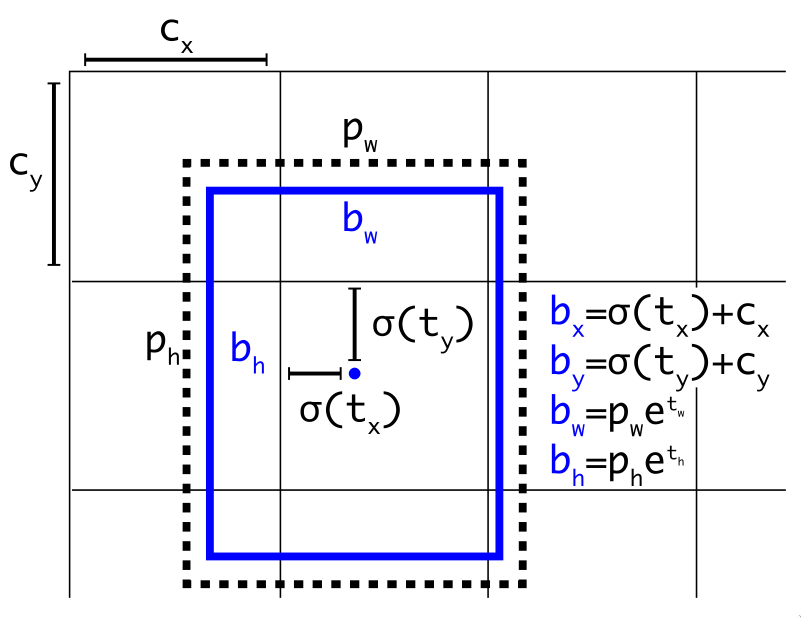
\includegraphics[width=6cm]{imgs/bbox_calculation.png}
    \caption{Final bounding box calculation in the YOLOv4 network based on an anchor box \cite{yolov2}}
    \label{fig:bbox_calculation}
\end{center}
\end{figure}

\subsubsection{Loss}

\ac{YOLO} is trained end-to-end and requires to predict the class as well as the bounding boxes a multi-task loss.
The loss can be separated into three main parts:

\begin{enumerate}
    \item class loss
    \item objectness loss
    \item bounding box regression loss
\end{enumerate}

In the following $1_{sb}^{obj}$ denotes that the anchor box $b$ in grid cell $s$ is responsible for detecting the object.
Before training responsibility is assigned by making that anchor box responsible which has the highest \ac{IoU} with the ground truth bounding box.
Furthermore, $S^2$ denotes the number of grid cells in a particular scale and $B$ and the number of anchor boxes present in a grid cell.
All predicted values are denoted with a ``hat'' (e.g. $\hat{P}$).

The class loss (eq. \ref{eq:yolo_lclass}) is calculated by taking the sum of all possible anchor boxes and the sum of all independent class losses, which is calculated with the \ac{CE} Loss.
An anchor box only contributes to the loss, when an object is labeled to be present in it.

\begin{equation}
    L_{class} = \sum_{s=0}^{S^2} \sum_{b=0}^B \sum_{c \in classes} 1_{sb}^{obj} * CE(P_{sbc}, \hat{P}_{sbc})
    \label{eq:yolo_lclass}
\end{equation}

The bounding box regression loss (eq. \ref{eq:yolo_lbbox}) is calculated again as the sum of all possible anchor boxes, taken over an \ac{IoU} based loss function denoted as XIoU (e.g. \ac{IoU}, \ac{GIoU}, \ac{DIoU}, \ac{CIoU}, \ac{EIoU}).
Additionally, the XIoU is multiplied with a scaling weight which enforces a multiplier based on the size of the ground truth bounding box, i.e. if the bounding box is small more weight is applied on the loss of that bounding box.

\begin{equation}
    L_{IoU} = \sum_{s=0}^{S^2}\sum_{b=0}^{B} 1^{obj}_{sb} * w_{scale} * XIoU(bbox, \hat{b}box)
    \label{eq:yolo_lbbox}
\end{equation}

\begin{equation}
    w_{scale} = 2 - w * h
\end{equation}

The last part of the multi-task loss is the objectness loss, where objectness is defined as the confidence of the network that an object is present in a grid cell or not.
The objectness loss is split into two sub equations.
The former (eq. \ref{eq:yolo_lobj}) defines the loss which occurs when an object is present and the latter (eq. \ref{eq:yolo_lnoobj}) when no object is present.
Again, both are taken over the sum of all possible anchor boxes.
$L_{obj}$ takes the sum of all \ac{CE} Loss outputs, applied to $1_{sb}^{obj}$ and the predicted objectness score.
Almost the same is done in $L_{noobj}$, but instead here the inverse prediction score is used.
Additionally, a constraint is introduced that makes the loss only contribute when the maximum \ac{IoU} of the predicted and any ground truth bounding box is below a certain threshold $t_{ignore}$.
This does not penalize predictions which have a high \ac{IoU}, but should normally not be present, i.e. another anchor box is assigned as a predictor.
For example this can happen when during prediction responsibility assignment two anchor boxes had a similar \ac{IoU} with the ground truth bounding box, the network hence tries to predict both of them.

\begin{equation}
    L_{obj} = \sum_{s=0}^{S^2}\sum_{b=0}^{B} CE(1^{obj}_{sb}, \hat{P}_{sb})
    \label{eq:yolo_lobj}
\end{equation}

\begin{equation}
    L_{noobj} = \sum_{s=0}^{S^2}\sum_{b=0}^{B} CE(1^{noobj}_{sb}, 1 - \hat{P}_{sb}) * \{max(IoU(\forall bbox, \hat{b}box_{sb})) < t_{ignore}\}
    \label{eq:yolo_lnoobj}
\end{equation}


Finally, each of the above losses is multiplied with a tunable hyperparameter and summed up to form the final \ac{YOLO} loss.

\begin{equation}
    L_{YOLO} = \lambda_{class} * L_{class} + \lambda_{IoU} * L_{IoU} + \lambda_{objectness} * (L_{obj} + L_{noobj})
    \label{eq:yolo_loss}
\end{equation}

\subsubsection{Non-Maximum Suppression}

During prediction time often multiple bounding boxes are predicted for one object.
To deal with this and suppress unnecessary bounding boxes a \ac{NMS} algorithm is applied.
More precisely \ac{DIoU}-\ac{NMS} \cite{diou}, since it has shown to perform better than classical \ac{NMS} \cite{soft_nms}, especially in cases of occlusion.

In the following the algorithm for \ac{DIoU}-\ac{NMS} is presented.
The input is a set of bounding boxes $B$ as well as the corresponding prediction scores $S$ and a suppression threshold $\epsilon$.
The algorithm first selects the bounding box $B_m$ with the highest score $S_m$ and compares it to every other bounding box $b_i$ in the set.
If the \ac{DIoU} measure between $B_m$ and $b_i$ is above the threshold $\epsilon$, the bounding box $b_i$ gets suppressed by removing it from the set $B$.
This process is repeated until no bounding boxes are present in $B$.

\begin{algorithm}[caption={DIoU-NMS Algorithm TODO caption to bottom and format}, label={alg1}]
input: $B$ = {$b_1$,...,$b_N$}, $S$ = {$s_1$,...,$s_N$}, $\epsilon$
       $B$: list of bounding box proposals
       $S$: list of bounding box scores
       $\epsilon$: NMS threshold
output: $B_S \subseteq B$, $B_S = \{b_1,...,b_M\}$
        $B_S$: list of bounding boxes after suppression
        $S_S$: list of bounding box scores after suppression

begin
$B_S \gets \{\}$; $S_S \gets \{\}$
while $B \neq empty$ do
    $m \gets$ argmax($S$)
    $B_m \gets B[m]$; $S_m \gets S[m]$

    $B_S \gets B_S \cup B_m$; $S_S \gets S_S \cup S_m$
    $B \gets B - B_m$; $S \gets S - S_m$

    foreach $b_i$, $s_i$ in $B$, $S$ do
        if $DIoU(B_m, b_i) \geq \epsilon$ then
            $B \gets B - b_i; S \gets S - s_i$
        end
    end

    return $B_S$, $S_S$
end
\end{algorithm}
